\begin{multicols*}{2}
The udacity dataset is created from the udacity car simulator. It associate via a timestamp 3 images taken at an offset (left, center and right) with steering angles, brake and acceleration. Our dataset contains 8036 frames of the simulation game along with odometry information. These images have been resized and modified in the following way randomly in order to increase the model’s prediction capacity: 
\begin{itemize}	
	\item Randomly chosen from an offset (left, center, right)
	\item Brightness changed
	\item Cropped
	\item Shadow mask added
	\item Flipped (left becomes right and right becomes left)
	\item Translated (shift the image vertically and horizontally)
	\item RGB 2 YUV (YUV is a color space more closely related to human perception)
\end{itemize}
All of the preprocessing is done using the python opencv library.
\\
\begin{minipage}{.25\textwidth}
	\centering
	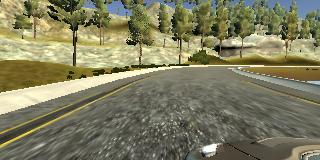
\includegraphics[width=0.2\linewidth]{images/left_image.png}
	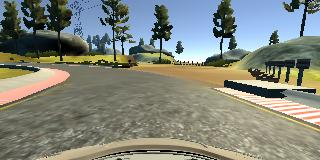
\includegraphics[width=0.2\linewidth]{images/center_image.png}
	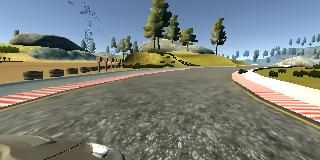
\includegraphics[width=0.2\linewidth]{images/right_image.png}
	\captionof{figure}{Left, Center and Right Image}
\end{minipage}
\end{multicols*}